\section{Example: Tracking through Magnetic Fields}

This examples illustrates the tracking mechanism of \W (and by the way
the use of the command line{\ldots} for the plotting.) After

~~~~~\senv

We start from
\we and use the python script
\gtis{../python/wave\_example\_2.py}
to create \wie. But before, we have a look on it. We open
\gtis{../python/wave\_example\_2.py} with an text editor (Fig. \ref{ex2fig1}):

\begin{figure}[htb]
    \centering
    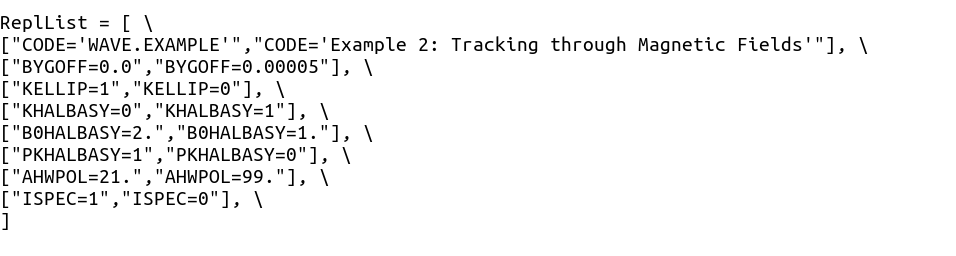
\includegraphics[width=0.9\textwidth]
    {pics/wave_example_2_py.png}
    \caption{First part of the script to set-up \textit{wave.in} for the second example
    \textit{wave.out}}
    \label{ex2fig1}
\end{figure}

The list \gtis{ReplList} contains the strings to be replaced in \wie. Each
line contains two strings. The first string
in \wi is replaced by the second.
Most of the variables you known from example 1,
but the variable
\ispec belonging to the namelist \contrl is new.
Changing \ispecone to \ispecnull, switches the spectrum
calculations off. Also new is the variable \gtis{BYGOFF}, which is a
global field offset added to the undulator field, e.g. to simulate the
earth field.

Now we execute the script,
copy the resulting file, and run \W:\\

\cboxs{
python3 ../python/wave\_example\_2.py \\
cp ../input/wave\_example\_2.in wave.in \\
wave\\
}

On the terminal, two warnings appear, indicating that the trajectory
is not correctly adjusted. This means, a final kick and a final offset
remain. We start the plotting GUI:

\cboxs{wplot\\}

Click the button \gtis{Plot}, select \gtis{Overview}, and check the results.

We see in the overview Fig. {\ref{ex2fig2}} that
the trajectory is distorted as expected due to the external field,

\begin{figure}[htb]
    \centering
    %\framebox(12,9){
      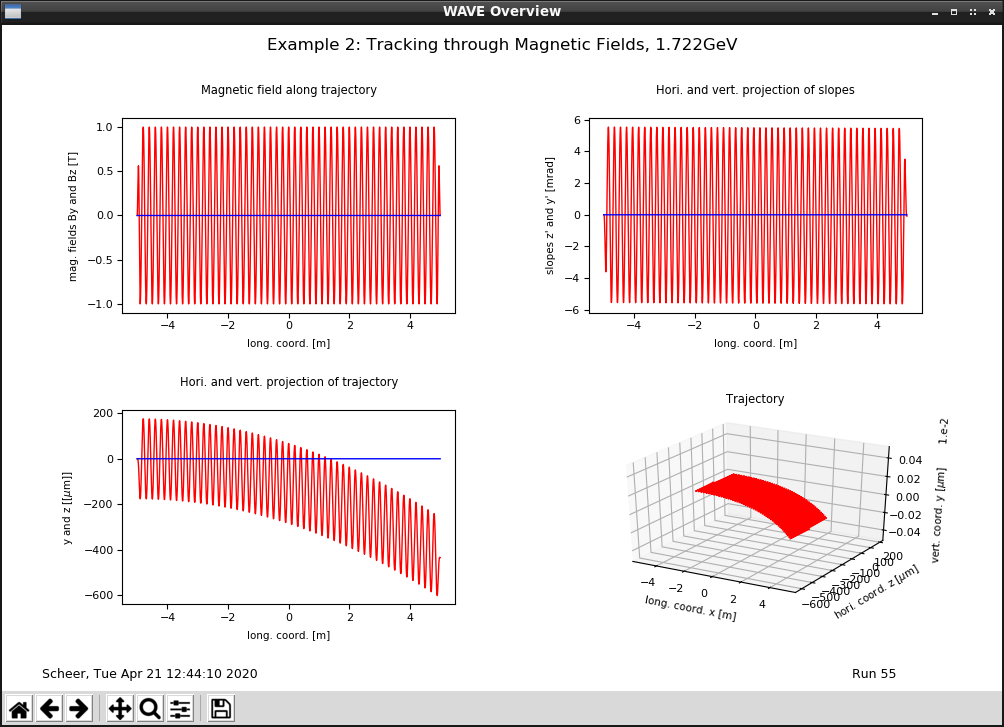
\includegraphics[width=0.7\textwidth]
      {pics/trajectory_ex2.png}
    %}
    \caption{The trajectory with \gtis{XINTER=-9999.}}
    \label{ex2fig2}
\end{figure}

Sometimes, it's useful to adjust the trajectory, e.g. if you want to have
a symmetric one with respect to the center of the straight section or
if for a given field model the correct endpole constellation is
missing. This can be achieved with by tuning the electron parameters in the
namelist \contrle:

The most interesting variable is \gtis{XINTER}, which defines the
x-coordinate the other variables like \ystart or \vzin refer to.

Edit \wie and set

\cboxs{XINTER=0.}

Then we save the file and enter:

\cboxs{wave \\
wplot \\
nz()
}\\

and see (Fig. \ref{ex2fig4}) a trajectory, where the electron passes the origin with zero
slope according to:

\begin{figure}[htb]
    \centering
    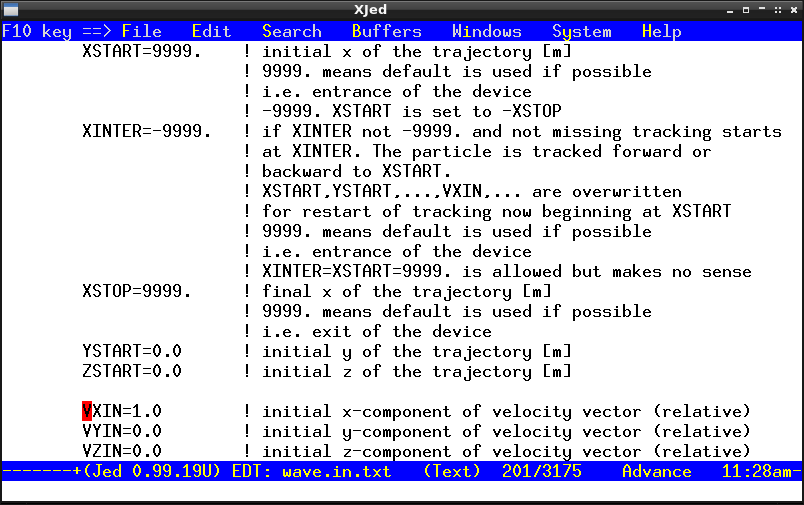
\includegraphics[width=0.8\textwidth]
    {pics/ex2_xinter.png}
    \caption{Electron variables}
    \label{ex2fig3}
\end{figure}

\cboxss{
\bsp ~YSTART=0.\\
ZSTART=0.\\
VXIN=1.\\
VYIN=0.\\
VZIN=0.
}

at

\cboxss{XINTER=0.}

Thus, if \scap{XINTER} is not \gtis{-9999.}, WAVE tracks
first the electron from \scap{X = XINTER} back to
\xstart and then starts the actual tracking through the magnetic
field.

You can save the picture with
the corresponding toolbar button or typing ''s'' when the cursor is
over the plotting window or by typing e.g.

\cboxs{pplot("trajectory.png")}\\
or

\cboxs{pplot("trajectory.pdf")}

in the Python shell. (If the overview is plotted a file \scap{
WaveOverview.pdf} is written automatically.) The last plotting command \\

 \cboxs{nz()}

can of course also be triggered from the GUI menu. The ''n'' referes
to the fact, that the data stem from an n-tuple. You can also try \\

 \cboxs{nby()}

and so on. You might have alread noticed, that the plotting commands
executed by the GUI are echoed in the Python shell.
The command echoes show you
the syntax and parameters of the plotting commands applied. So you can
learn short-cuts for plotting from the Python shell.

If you don't see these command echos,
the configuration file \gtis{waveplot.cfg} is missing in your working
directory. You find an example in the input-directory \gtis{\$WAVE/input}.

If \gtis{waveplot.cfg} is present, plotting options are read from this
file. E.g. you can set the window size, trigger
saving of all plots or writing plotted
data to ASCII-Files. To see all options, check this file.

Some options can also be toggled in the GUI or by commands, e.g.

 \cboxs{optecho(1)}

 or

 \cboxs{optecho(0)}

 or

 \cboxs{optstat(1)}

 or

 \cboxs{optstat(0).}


\begin{figure}[htb]
    \centering
    %\framebox(12,9){
    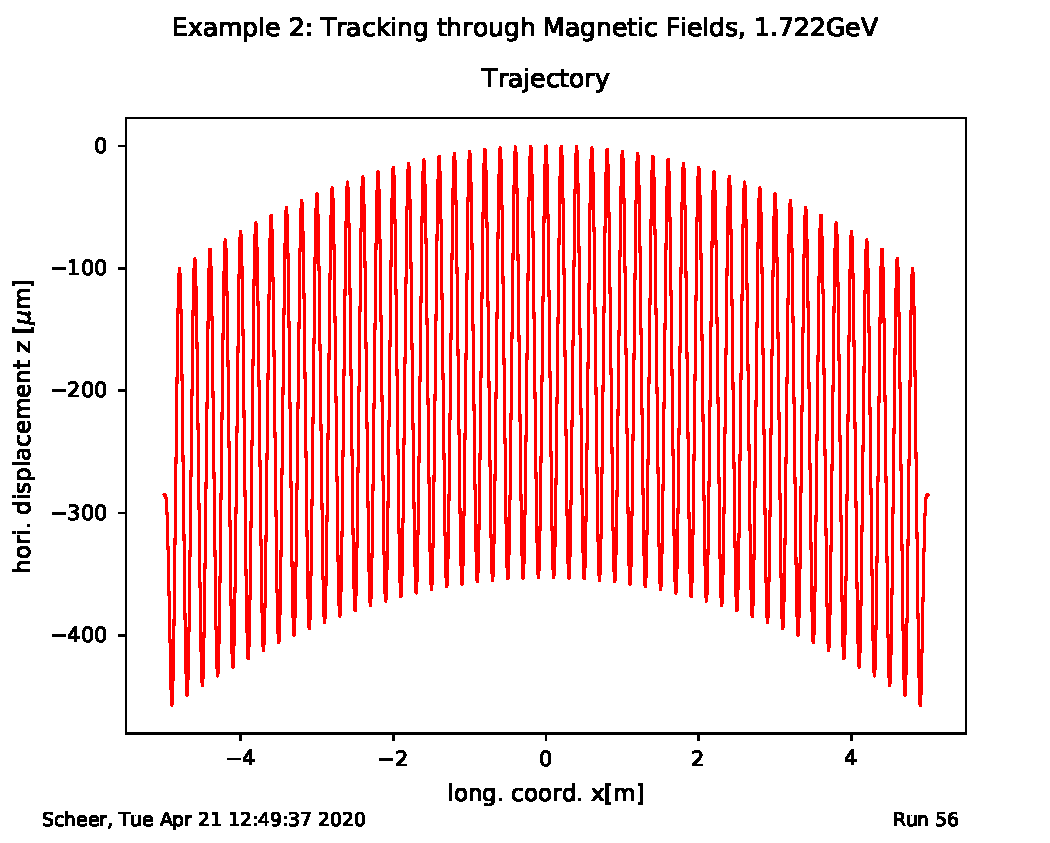
\includegraphics[width=0.7\textwidth]
    {pics/ex2_xinter_0.pdf}
    %}
    \caption{Adjusted trajectory with \gtis{XINTER=0.}.}
    \label{ex2fig4}
\end{figure}

Note: If you calculate synchrotron radiation from this trajectory,
i.e. \ispecone, the
back tracking at the beginning does, of course, not contribute to the
radiation or irradiated power of the device. By the way, this power is
given in the output
file \woe. The power is normalized to the beam current
\dmycurr in the namelist \contrl. In \wo you also find the energy loss
of the electron having passed the magnetic field. This is controlled by
\ieneloss also namelist \contrl. For very long undulators or
wigglers, the energy loss influcences the trajectory and the spectrum
of synchrotron radiation. For a single, typical insertion devices,
this can be neglected, i.e. \ienelossnull can be used.
